\chapter{Experiments and Results}
\com{
\todo[inline]{
Sometimes this is split into two chapters.\\

Keep in mind: How you are going to evaluate what you have done? What are your metrics?\\
Analysis of your data and proposed solution\\
Does this meet the goals which you had when you started?
}
}
\label{ch:results}

DRAFT

\noindent
The results obtained from the localisation and mapping feature added to the \gls{ALM} are shown.


\section{Localisation Analysis}
\label{sec:locRes}
\noindent Analysis of the Simulated and Outdoor Experiment.
Real Test configuration and environment in outdoor settings.

Test on real measurements gathered in different conditions of terrain, slope, and weather.
Multiple tests have been repeated to measure the measurement's value noise of each sensors.


\begin{table}[!ht]
	\small
	\begin{center}
		\label{tab:eval}
		\begin{tabular}{|c||c|c|c|c|c|c|c|}
			\hline
			\multirow{2}{*}{\textbf{Model}} & \multicolumn{6}{c|}{\textbf{Sensors}} & \multirow{2}{*}{\textbf{Comment}}\\
			& \multicolumn{1}{c|}{Control} & \multicolumn{1}{c|}{\gls{WO}} & \multicolumn{1}{c|}{\gls{GNSS}}& \multicolumn{1}{c|}{\glspl{GNSS}} & \multicolumn{1}{c|}{\glspl{IMU}} & \multicolumn{1}{c|}{\gls{VO}} & \\
			\hline
			\hline
			\centering{1} & YES & YES & YES & NO & NO & NO & Original \\
			\hline
			\centering{2} & YES & YES & YES & YES & YES & YES & Complete \\
			\hline
			\centering{3} & YES & YES & YES & NO & YES & YES & Reliable \\
			\hline
			\centering{4} & YES & YES & NO & NO & YES & NO & Cheap solution \\
			\hline
			\centering{5} & YES & NO & YES & NO & NO & YES & -WO+VO \\
			\hline
			\centering{6} & NO & YES & YES & NO & YES & YES & No Control \\
			\hline
		\end{tabular}
		\caption{Experiments configuration}
	\end{center}
\end{table}

\subsection{Simulated Experiment }
\noindent The extensive and comprehensive experiment run with all the measures available is analysed here.

The following localisation performance have been obtained by the different configurations of sensors.

\begin{figure}[!ht]
	\begin{center}
		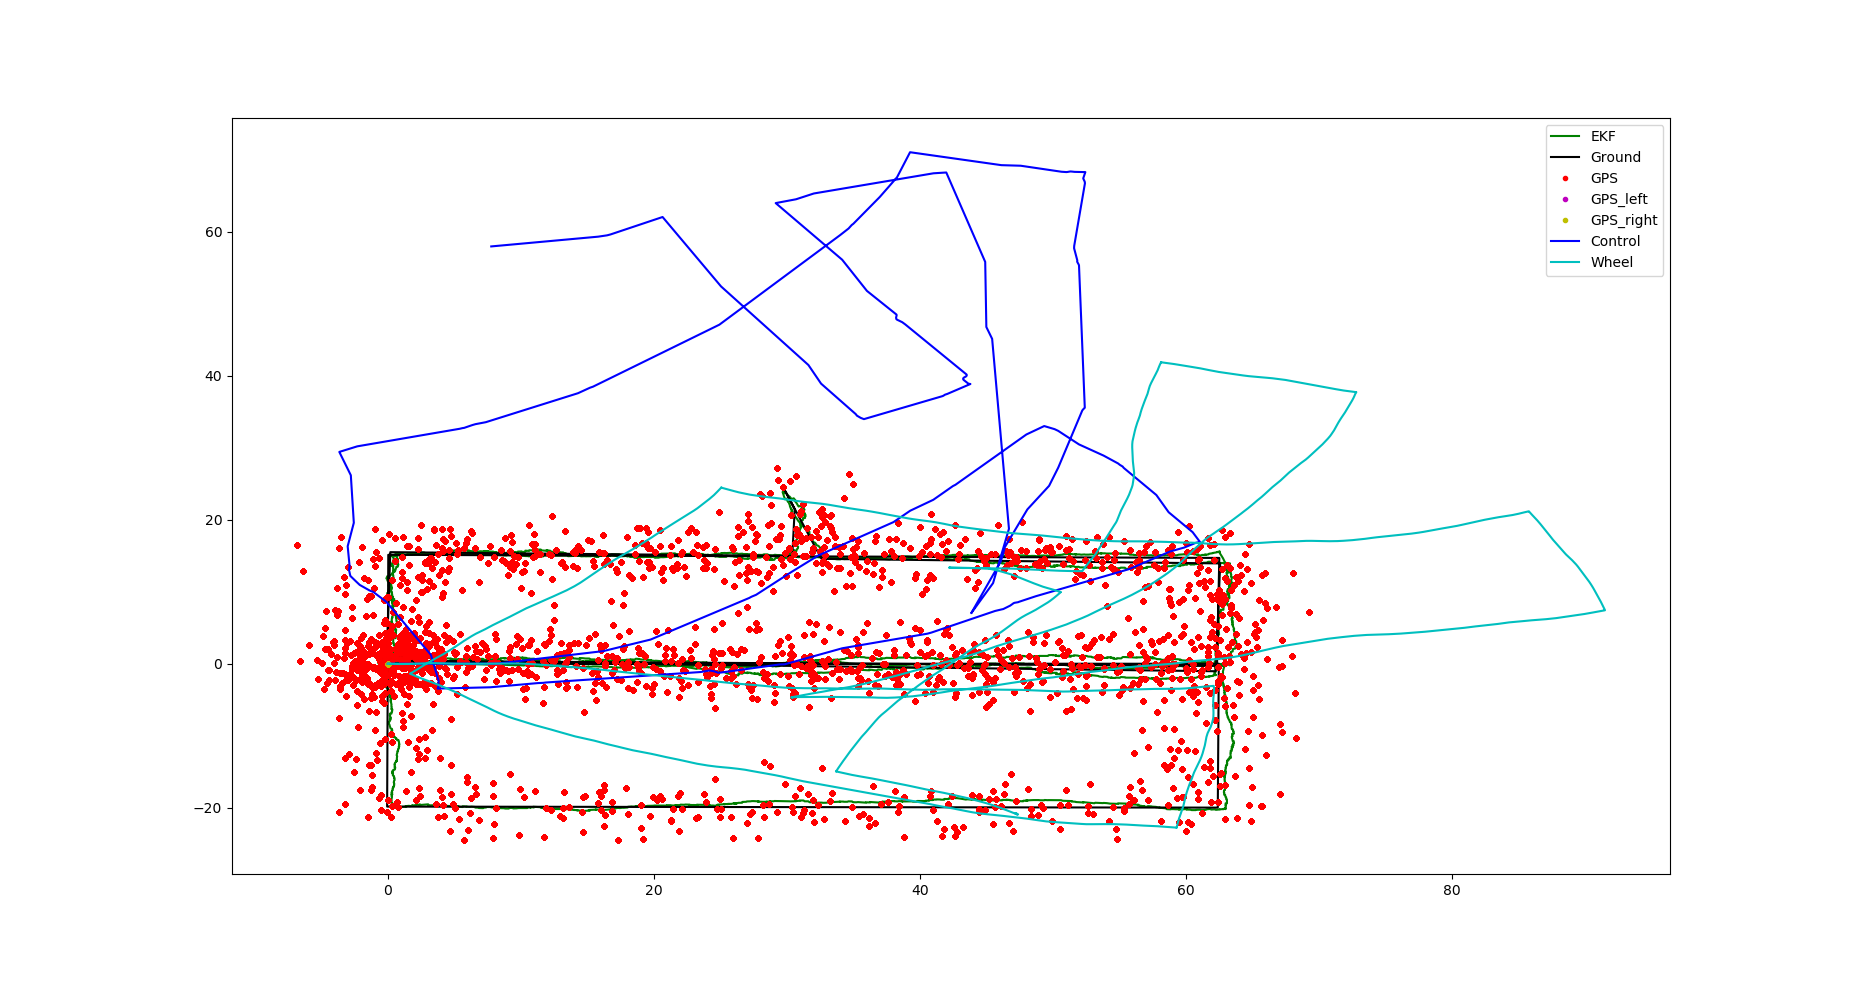
\includegraphics[width=1\textwidth]{Images/5-Results/Sim-Control-WO-GPSs-IMUs.png}
	\end{center}
	\caption{Simulation Experiment Results}
	\label{fig:simRes}
\end{figure}

These results have been evaluated using the \gls{RMSE} metric, the values obtained are showed in the Table below.


	\begin{table}[!ht]
		\small
		\begin{center}
			\label{tab:evalSim}
			\begin{tabular}{|c||S|S|S||S|S|S||S|S|}
				\hline
				\multirow{3}{*}{\textbf{Model}} & \multicolumn{8}{c|}{\textbf{Evaluation Criteria}} \\
				& \multicolumn{3}{c||}{\textbf{RMSE}} & \multicolumn{3}{c||}{\textbf{Uncertainty}} & \multicolumn{2}{c|}{\textbf{Time step}}\\
				& \multicolumn{1}{c|}{x[\SI{}{\meter}]} & \multicolumn{1}{c|}{y[\SI{}{\meter}]} & \multicolumn{1}{c||}{$\theta$[\SI{}{\radian}]} & \multicolumn{1}{c|}{x[\SI{}{\meter}]} & \multicolumn{1}{c|}{y[\SI{}{\meter}]} & \multicolumn{1}{c||}{$\theta$[\SI{}{\radian}]} & \multicolumn{1}{c|}{$\mu$[\SI{}{\milli \second}]} & \multicolumn{1}{c|}{$\sigma$[\SI{}{ms}]}\\
				\hline
				\hline
				\centering{Sim 1} & 4.35 & 4.10 & 0.6 & 10.35 & 5.10 & 1.6 & 4.23 & 0.1 \\
				\hline
				\centering{Sim 2} & 4.35 & 4.1 & 0.6 & 10.35 & 5.10 & 1.6 & 4.23 & 0.1 \\
				\hline
				\centering{Sim 3} & 4.35 & 14.10 & 0.6 & 10.35 & 5.10 & 1.6 & 4.23 & 0.1 \\
				\hline
				\centering{Sim 4} & 4.35 & 4.10 & 0.6 & 10.35 & 5.10 & 1.6 & 4.23 & 0.1 \\
				\hline
				\centering{Sim 5} & 4.35 & 4.10 & 0.6 & 10.35 & 5.10 & 1.6 & 4.23 & 0.1 \\
				\hline
				\centering{Sim 6} & 4.35 & 4.10 & 0.6 & 10.35 & 5.10 & 1.6 & 4.23 & 0.1 \\
				\hline
			\end{tabular}
			\caption{Simulated experiments results}
		\end{center}
	\end{table}


\subsection{Outdoor Experiment }
\noindent The extensive and comprehensive experiments run with all the measures available is analysed here.

The following localisation performance have been obtained by the different configuration of sensors.

\begin{figure}[!ht]
	\begin{center}
		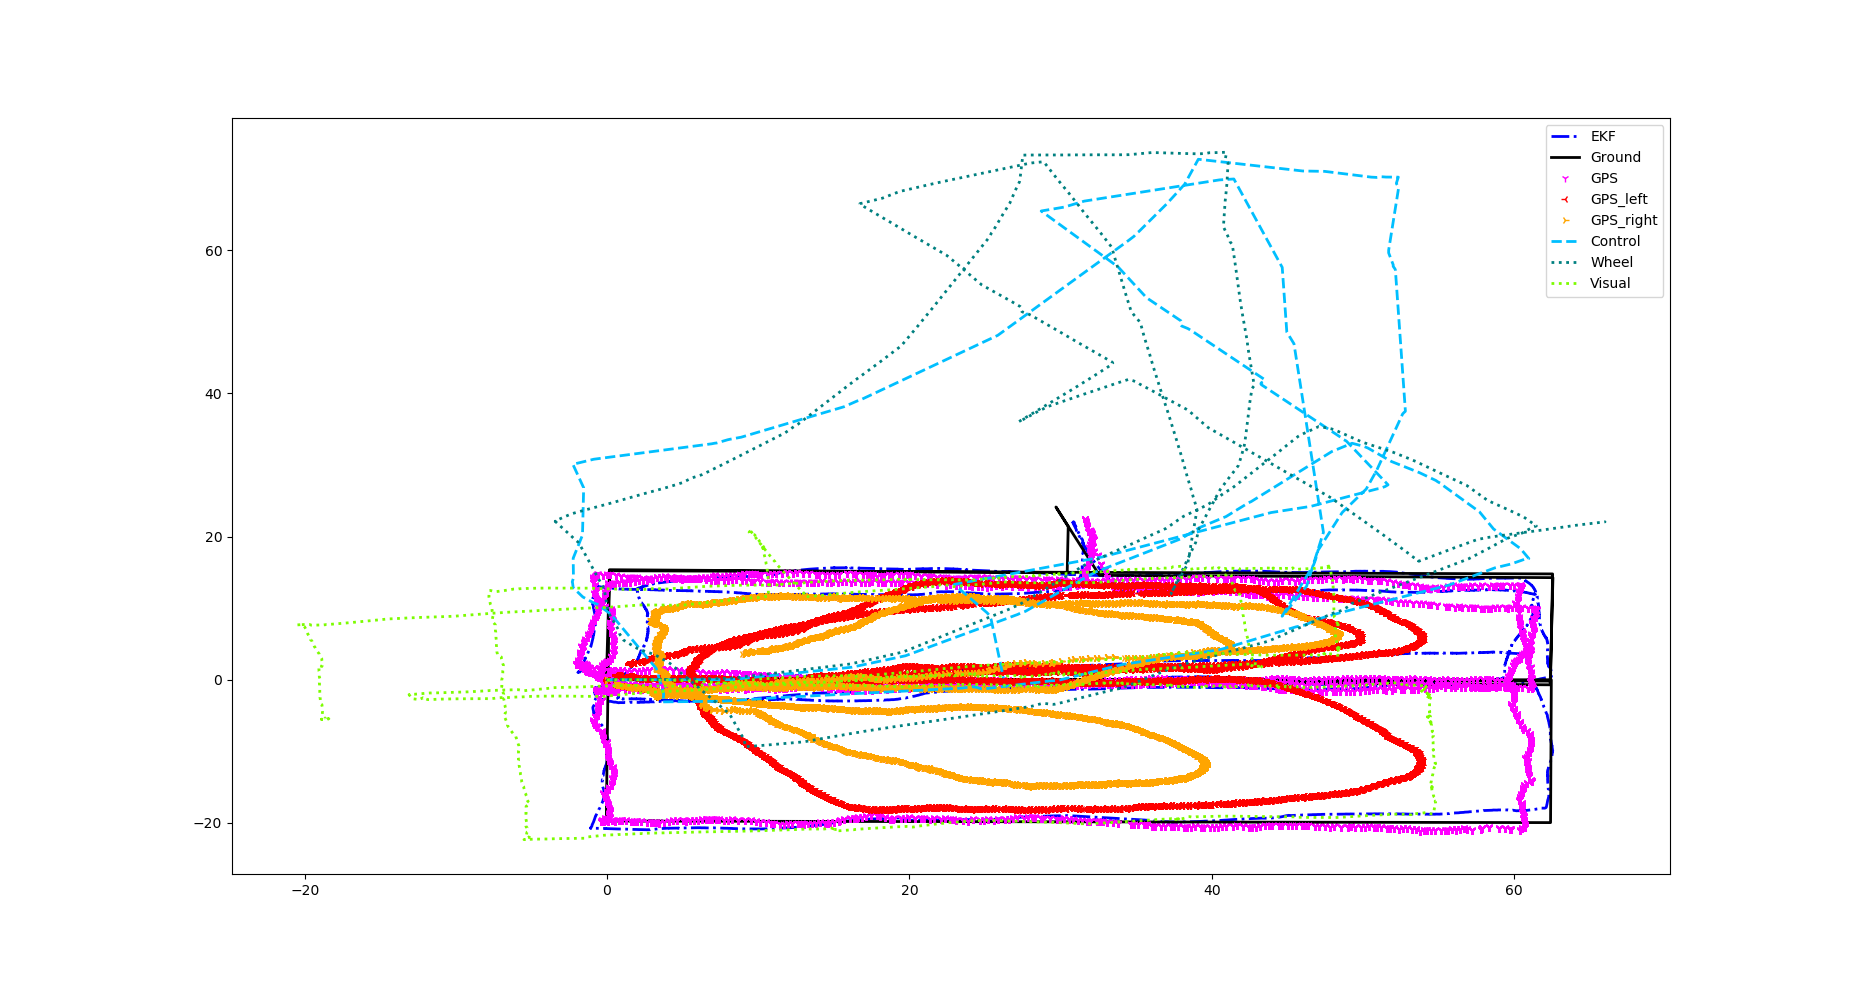
\includegraphics[width=1\textwidth]{Images/5-Results/Out-NoNMEA.png}
	\end{center}
	\caption{Outdoor Experiment Results}
	\label{fig:out}
\end{figure}

These results have been evaluated using the \gls{RMSE} metric, the values obtained are showed in the Table below.


	\begin{table}[!ht]
		\small
		\begin{center}
			\label{tab:evalOutdoor}
			\begin{tabular}{|c||S|S|S||S|S|S||S|S|}
				\hline
				\multirow{3}{*}{\textbf{Model}} & \multicolumn{8}{c|}{\textbf{Evaluation}} \\
				 & \multicolumn{3}{c||}{\textbf{RMSE}} & \multicolumn{3}{c||}{\textbf{Uncertainty}} & \multicolumn{2}{c|}{\textbf{Time step}}\\
				 & \multicolumn{1}{c|}{x[\SI{}{\meter}]} & \multicolumn{1}{c|}{y[\SI{}{\meter}]} & \multicolumn{1}{c||}{$\theta$[\SI{}{\radian}]} & \multicolumn{1}{c|}{x[\SI{}{\meter}]} & \multicolumn{1}{c|}{y[\SI{}{\meter}]} & \multicolumn{1}{c||}{$\theta$[\SI{}{\radian}]} & \multicolumn{1}{c|}{$\mu$[\SI{}{\milli \second}]} & \multicolumn{1}{c|}{$\sigma$[\SI{}{\milli \second}]}\\
				\hline
				\hline
				\centering{1} & 4.35 & 4.10 & 0.6 & 10.35 & 5.10 & 1.6 & 4.23 & 0.1 \\
				\hline
				\centering{2} & 4.3 & 4.10 & 0.6 & 10.35 & 5.10 & 1.6 & 4.23 & 0.1 \\
				\hline
				\centering{3} & 10.35 & 4.10 & 0.6 & 10.35 & 5.10 & 1.6 & 4.23 & 0.1 \\
				\hline
				\centering{4} & 4.35 & 4.10 & 0.6 & 10.35 & 5.10 & 1.6 & 4.23 & 0.1 \\
				\hline
				\centering{5} & 10.35 & 4.10 & 0.6 & 10.35 & 5.10 & 1.6 & 4.23 & 0.1 \\
				\hline
				\centering{6} & 4.35 & 4.10 & 0.6 & 10.35 & 5.10 & 1.6 & 4.23 & 0.1 \\
				\hline
			\end{tabular}
		\caption{Outdoor experiments results}
		\end{center}
	\end{table}

\section{Mapping Analysis}
\noindent The evolution of the mapping feature is defined here, from the initial setting, to the customised virtual boundary, and finally to the updating map behaviour.

The system adopted to localise the \gls{ALM} during this phase is "\textit{Model 2}" as defined in Section \ref{sec:locRes}


\subsection{Occupancy Grid Boundary}
\noindent
The virtual boundary is then set with the initial run setting of the personalized virtual boundary.
The external area is set to the outdoor limited area.

With this virtual boundary, the \gls{ALM} is able to stay within the designed area.

\begin{figure}[!ht]
	\begin{center}
		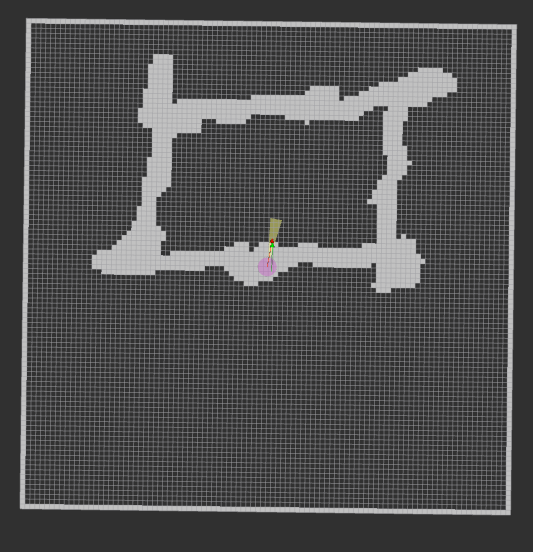
\includegraphics[width=0.75\textwidth]{Images/5-Results/BoundaryMap.png}
	\end{center}
	\caption{Personalised Boundary definition}
	\label{fig:occGridBoud}
\end{figure}


\subsection{Occupancy Grid Update}
\noindent
The virtual boundary is then set with the initial run setting of the personalised virtual boundary.


\begin{figure}[!ht]
	\begin{center}
		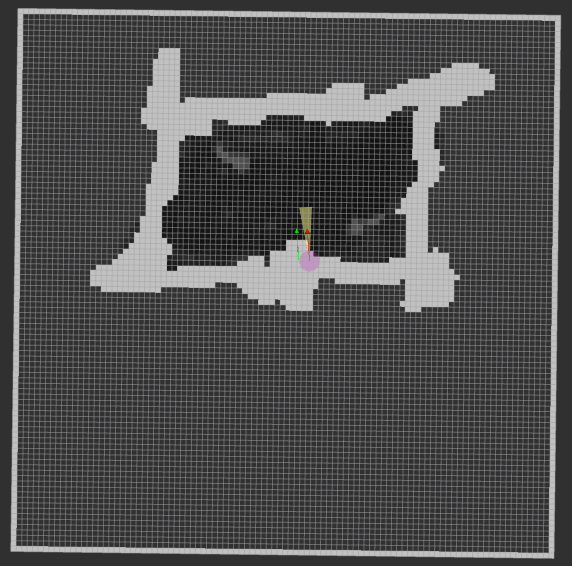
\includegraphics[width=0.75\textwidth]{Images/5-Results/CollisionMap.png}
	\end{center}
	\caption{Update of the map inside the boundaries (lighter shade means probability of object given by collision events)}
	\label{fig:occGridUpdate}
\end{figure}



%\section{Discussion}

\cleardoublepage
%\clearpage
